\section{Methods}
\label{sec:methods}


In what follows, we provide details on how we estimate the daily incident
infections for each state over the considered time period of June 1, 2020 to
November 29, 2021 and the data we used to achieve this.
\autoref{fig:cases_to_infect_flowchart} provides a visual summary of the data,
analysis tasks, and the relationships between them. The major analysis tasks
this figure aims to convey are as follows. First, we estimate variant-specific
incubation periods and two types of delay distributions for each day over the
time period under consideration. Next, each day-location-specific incubation
period and symptom onset to positive specimen delay distribution are combined
using convolution, resulting in variant-specific infection onset to positive
specimen distributions for each time and location (for a brief description of
convolution, please see \autoref{sec:convol}). Subsequently, two types of
deconvolution are performed. We first deconvolve from case report to positive
specimen date. We then deconvolve from positive specimen to report date by
variant. The resulting infection estimates are aggregated across the variant
categories and adjusted to account for the unreported infections by using
state-specific, time-varying seroprevalence data in an antibody prevalence
model. 


\begin{figure}[!tb]
\centering
    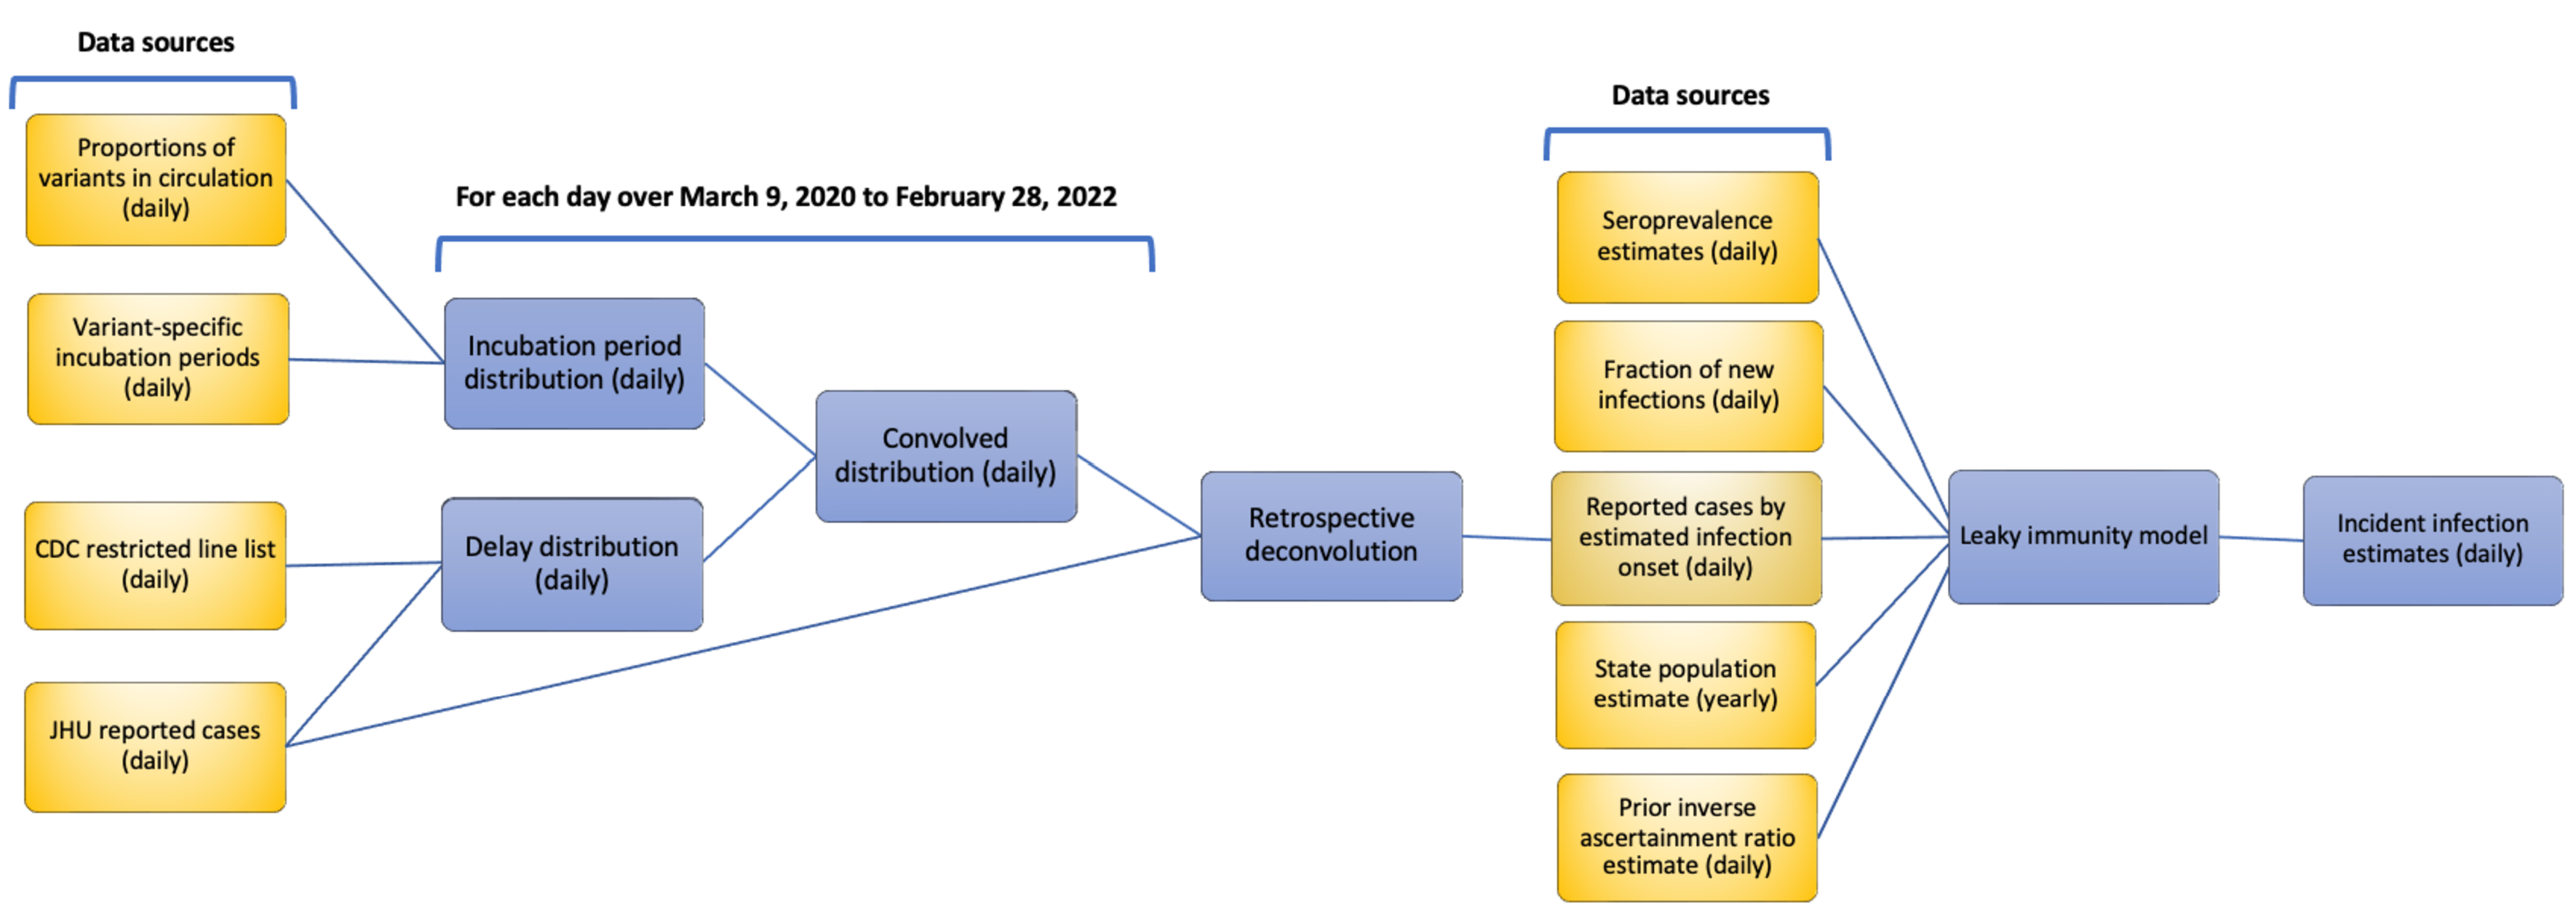
\includegraphics[width=.99\textwidth]{Reported_cases_to_infect_flowchart.pdf} 
    \caption{Flowchart of the inputted data and major analysis steps required to
    get from reported cases to incident infection estimates for each day over
    June 1, 2020 to November 29, 2021 for a state. Data sources are coloured in
    yellow, while data analysis steps are coloured in blue. The data sources
    that do not stem from an analysis step are literature estimates.}
    \label{fig:cases_to_infect_flowchart}
\end{figure}


% Reasons why we should start from June 1, 2020 
% A list of reasons on why I settled on these start and end dates: 
% 1. Reinfections officially started occurring 2020-06-01 according to the data we?re using
% 2. sero measurements start in July 2020 for most states or later
% 3. the prior values for the inverse of the ascertainment ratio estimates are as of 2020-06-01
% 4.  the earliest hospitalizations for each state (that we use in the correlation analysis) 
% are also almost always in July, 2020. 
% So I am not convinced we should extrapolate multiple months away from the start or end for sero. 
% One month in either direction seems reasonable & doesn't overreach.







\subsection{Estimating delay distributions from private line lists}
\label{sec:delaystop}

We obtain de-identified patient-level line list data on COVID-19 cases from the
CDC. Although there are both public and restricted versions of the dataset
available containing the same patient records \citep{cdc2020casepub,
cdc2020caserestr}, only the restricted dataset contains information on the state
of residence. The three key dates of interest are those for symptom onset,
positive specimen collection, and report to the CDC. Handling missingness and
imputation in these dates is somewhat complicated and so additional details and
justifications are deferred to \autoref{sec:linelist-details}.

We use the line list to estimate the delay distribution for the pairs symptom
onset to positive specimen and positive specimen to report. We provide the full
procedure for the latter, before giving a brief description below for the
former. First, define $z_{\ell,t}$ to be a case report occurring at time $t$ in
location $\ell$, and let $\pi_{\ell,t}(k)$ to be the probability that
$z_{\ell,t}$ has a positive specimen collected $k$ days earlier. We assume that
all positive specimens will be reported within 60 days and that no test will be
reported on the same date as it was collected, that is, $\pi_{\ell,t}(0) = 0$
and $\pi_{\ell,t}(k) = 0$ whenever $k > 60$. Let $N_{\ell,t}$ be the number of
$z_{\ell,s}$ with $s\in[t-75+1,t+60] = \mathcal{S}_t$ and positive specimen date
greater than $s-60$. Then, we first compute
\begin{align}
    \tilde{p}_{\ell,t}(k) = \frac{1}{N_{\ell,t}}\sum_{s \in \mathcal{S}_t}
    \big(\textrm{\# $z_{\ell,s}$ with positive specimen at $s-k$}\big).
\end{align}
Next we compute a similar national quantity $\tilde{p}_{t}(k) =
\frac{1}{N_{t}}\sum_{s \in \mathcal{S}_t} \big(\textrm{\# $z_{s}$ with positive
specimen at $s-k$}\big)$, without restricting to location $\ell$. Next, let
$\alpha_{\ell,t}$ be the ratio of $N_{\ell,t}$ to the number of cases reported
by JHU CSSE\cite{dong2020interactive} in the same window. Then, compute
$p_{\ell,t}(k) = \alpha_{\ell,t}\tilde{p}_{\ell,t}(k) +
(1-\alpha_{\ell,t})\tilde{p}_t(k)$. This construction allows for more reliance
on the state estimate when there are more CDC cases relative to JHU (and vice
versa). We calculate the mean $m_{\ell,t}$ and variance $v_{\ell,t}$ of
$\{p_{\ell,t}(k) : 0<k\leq 60\}$ and estimate a gamma distribution by solving
the moment equations $m_{\ell,t} = \alpha_{\ell,t}\theta_{\ell,t}$ and
$v_{\ell,t}= \alpha_{\ell,t}\theta_{\ell,t}^2$ for the shape $\alpha_{\ell,t}$
and scale $\theta_{\ell,t}$. Finally, we discretize the resulting gamma density
to the support set of 1 to 60 days to produce an estimate
$\{\widehat{\pi}_{\ell,t}(k): 0 < k \leq 60\}$ of the delay distribution
$\pi_{\ell,t}$.
 
Estimating the delay from symptom onset to positive specimen date follows the
same procedure with a few minor adjustments. First, we allow $k$ to range from
$-3$ to $21$ (rather than 1 to 60). These upper and lower bounds are based on
the largest delay values for the state-wide 0.05 and 0.95 quantiles. This is
reasonable because the median delay is very short at approximately 2 days, and
an asymptomatic individual may test positive following a known exposure, before
the onset of symptoms. Additional minor details are discussed in
\autoref{sec:delay-justifications}.



\subsection{Estimating the incubation period distributions} 
\label{sec:incubation}

To account for the incubation period, the time between infection and symptom
onset, we use estimates from the existing literature, modified slightly for
coherence with each other: we model each incubation as a gamma distribution with
different parameters. We focus on the following eight variants, which dominated
at various points during our study period: Ancestral/Other, Alpha, Beta, Epsilon,
Iota, Gamma, Delta, and Omicron. Alpha, Beta, Delta, Gamma, and Omicron are all
variants of concern \citep{who2021tracking}, while we include the Epsilon
(California) and Iota (New York) variants because of large impact on those and
neighbouring states \citep{yang2022investigation, duerr2021dominance}.

The Ancestral variant has been modelled as a gamma distribution
\citep{tindale2020evidence}, so we simply use the reported shape and scale parameters. For the
Alpha, Beta, Gamma, Delta and Omicron variants, we use the reported mean and
standard deviation of the number of days of incubation \citep{tanaka2022shorter,
grant2022impact, ogata2022shorter}. To match these moments to the gamma
distribution, we solve the same moment equations described in
\autoref{sec:delaystop}. Then, we discretize each resulting density shown in \autoref{fig:inc_gammas} to the
support set, which is taken to be from 1 and 21 days. This range assumes that
symptoms require at least 1 day to develop \citealp{phcan2021covid} and that an
asymptomatic infection will resolve within 21 days
\citep{zaki2021estimations,cortes2022sars}.

We were unable to locate incubation period estimates for the geo-specific
Epsilon and Iota variants, so we use the incubation period for Beta because
Epsilon, Iota, and Beta are all children from the same parent in the
phylogenetic tree of the Nextstrain Clades \citep{hodcroft2021covariants}. All
other circulating variants are grouped together with the Ancestral variant.
There was little available sequencing data prior to Alpha-emergence, but
unfortunately, later in the pandemic, it is impossible to separate Ancestral
from other rare variants (which is one reason why we may refer to it as the Other category).

\begin{figure}[!tb]
\centering
    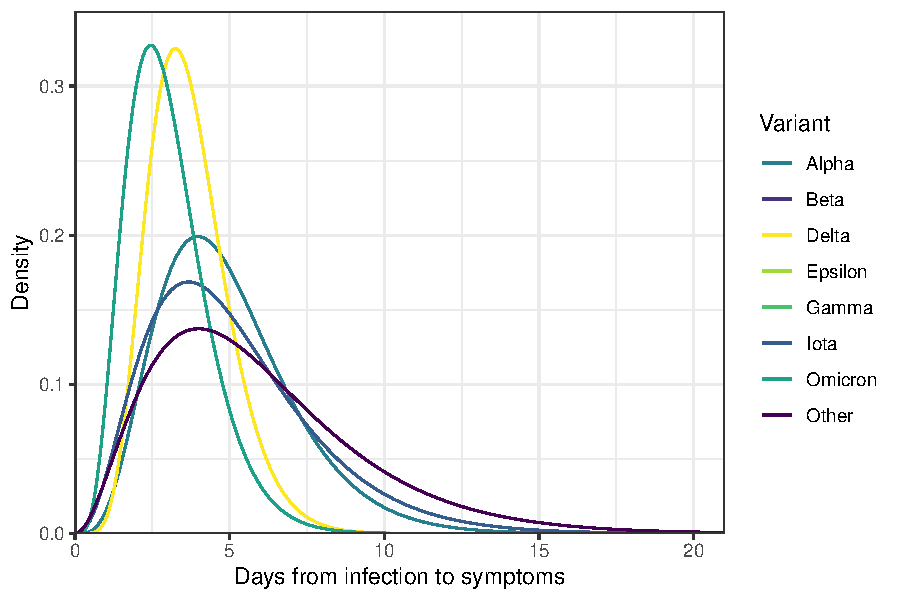
\includegraphics[width=0.6\linewidth]{inc-gammas-1.pdf}
    \caption{Gamma density for the incubation period of each of the eight
    variant categories. Note that the Ancestral variant directly utilizes the
    available gamma shape and scale parameters, while the remaining variants use
    the method of moments to estimate the gamma parameters.}
    \label{fig:inc_gammas}
\end{figure}

\subsection{Variant circulation proportions}
\label{sec:variant-proportions}

To estimate the daily proportions of the variants circulating in each state, we
obtain the GISAID genomic sequencing data from CoVariants.org
\citep{hodcroft2021covariants, elbe2017data}. These counts represent the total
number of cases belonging to a particular variant using
a sample of positive tests over a biweekly period. To estimate the population
proportion of each variant, we apply multinomial logistic regression 
for the eight variant categories separately for each state.

We let $V_{j\ell,t}$ to be the probability of a new cases at time $t$ in location
$\ell$ corresponding to variant $j$. Let $v_{j\ell,t}$ be the analogous observed
proportion. Then the nonparametric multinomial logistic regression model is given
as the system
\begin{equation}
\log\left(\frac{V_{j\ell,t}}{1-V_{j\ell,t}}\right) = f_{j\ell}(t),\;\; j=1,\ldots J,\quad
\textrm{subject to }\sum_{j=1}^J \exp\{f_{j\ell}(t)\} = 1, \;\;\forall t.
\end{equation}
The constraint ensures that the estimated proportions will sum to 1 across all
$J$ variants. To encourage smoothness of the estimated proportions, we specify
$f_{j\ell}(t)$ as a third-order polynomial in time: that is $f_{j\ell}(t) =
\beta_{j\ell,0} + \beta_{j\ell,1} t + \beta_{j\ell,2}t^2 + \beta_{j\ell,3}t^3$,
computed such that the resulting matrix of covariates is orthogonal.
 \autoref{fig:prop_figs} shows the proportions by variant for California before
(left) and after (right) the smoothing procedure. 

\begin{figure}[!tb]
\centering
    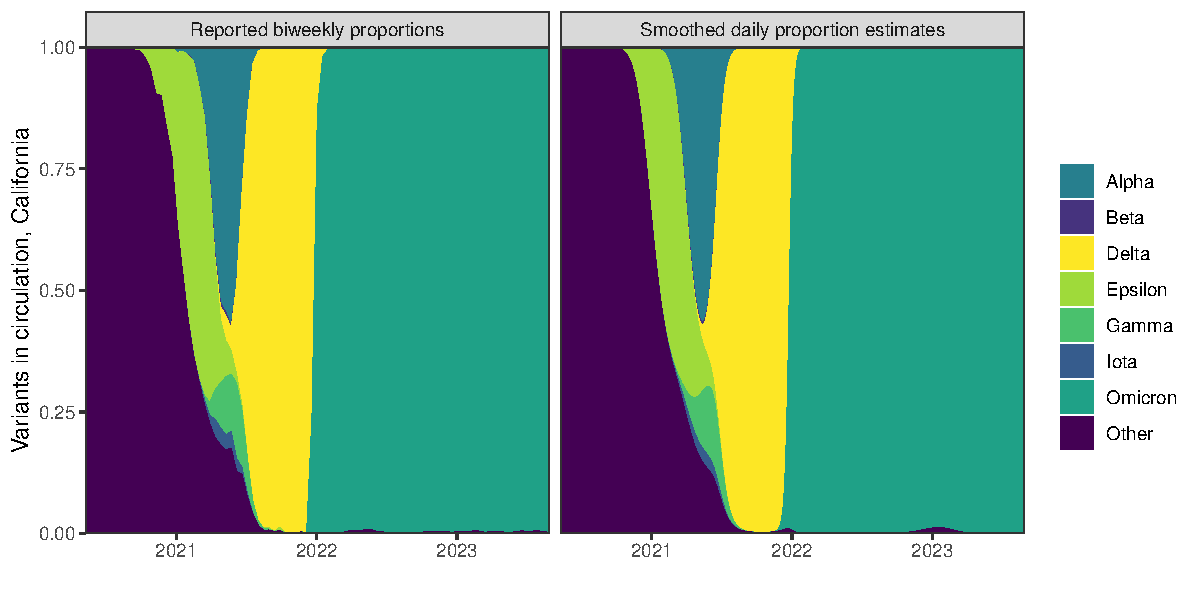
\includegraphics[width=\linewidth]{var-props-1.pdf}
    \caption{Left: Original biweekly proportions of the variants in circulation
    for California. Right: Daily proportions of the variants in circulation for
    California.}
    \label{fig:prop_figs}
\end{figure}

\subsection{Retrospective deconvolution: from cases to infections}
\label{sec:deconvolution}

Retrospective deconvolution estimates the daily number of new infections
corresponding to each variant for each time and location, ``pushing back'' the
dates that those cases were eventually reported to the time of infection.
Because the circulating variant proportions in \autoref{sec:variant-proportions}
correspond to the positive specimen date, this requires two stages. The first is
the deconvolution from report to positive specimen date, and the second is from
positive specimen date to infection onset date.

An important aspect of our methods is that deconvolution is not the same as a
shift. Simply shifting cases back in time and increasing them by some
factor fails to capture the temporal dynamics of the pandemic. In our
situation, reported cases are ``pushed back'' by the delays shown in
\autoref{fig:chain_events_onset_report}. 

We will start by describing the first type of deconvolution performed from
report to positive specimen date in detail. For this problem, let $t=1,\ldots,T'$
index the extended deconvolution period from March 1, 2020 to March 1, 2023,
extended to minimize the effects of boundary issues. \attn{Ryan, thoughts on
this notation? The sum over $t$ is awkward.} Define $y_{\ell,t}$
to be the number of new cases reported in location $\ell$ at time $t$, as
reported by the John Hopkins Center for Systems Science and Engineering (JHU
CSSE)\citealp{dong2020interactive} and retrieved with the The COVIDcast API
\citep{reinhart2021open}. Recall that $\widehat{\pi}_{\ell,t}(k)$ is the
associated probability that these reported cases were collected $k$ days earler. 

We estimate the deconvolved cases by positive specimen date by solving the
following optimization problem:
\begin{align}
\minimize_{\mathbf{x}}\ \sum_{t=1}^{T'} 
\left( y_{\ell,t} -  \sum_{k=1}^{60}\widehat{\pi}_{\ell,t}(k) x_{t-k} \right)^2 
+ \lambda\ \sum_{t=4}^{T'} \big|x_t - 4x_{t-1} + 6x_{t-2} -4x_{t-3}+ x_{t-4}\big|.
\end{align}

The two parts of this optimization problem trade data fidelity (the sum of
squared errors) with smoothness in the resulting estimates (the absolute error
of the differences of $\mathbf{x}$). The tuning parameter $\lambda$ determines
the relative importance of these competing goals. The solution to the problem is
an adaptive piecewise cubic polynomial \citep{tibshirani2014adaptive,
tibshirani2022divided} and can be accurately computed with ease
\citep{ramdas2016fast}. We select $\lambda$ with $3$-fold cross validation
\citep{jahja2022real} in which every third day is reserved for testing, and the
value that results in the smallest out-of-sample mean squared error is chosen.

The result of this first deconvolution is $\widehat{x}_{\ell,t}$, case estimates
by positive specimen date for each state. To continue, pushing back to infection
estimates, we first need the variant-specific delays from infection to positive
specimen collectio. These are calculated by convolving the
location-time-specific symptom-to-test distributions from
\autoref{sec:delaystop}, denoted by $\{q_{\ell,t}(k) : -3\leq k \leq 21\}$, with
the variant-specific incubation periods from \autoref{sec:incubation}, denoted
by $\{i_{j}(k) : 0 < k \leq 21\}$. The convolution of these yields a
distribution $\mathbf{q}_{\ell,t}*\mathbf{i}_j = \{\tau_{j\ell,t}(k): -3 \leq k
\leq 42\}$. However, only a fraction of $\widehat{x}_{\ell,t}$ corresponds to
each variant, so we must weight them by the variant proportions
$\widehat{v}_{j\ell,t}$ estimated in \autoref{sec:variant-proportions}. The
analogous optimization problem is therefore:
\begin{align}
\minimize_{\mathbf{u}}\ \sum_{t=1}^{T'} 
\left( 
    \widehat{v}_{j\ell,t}\widehat{x}_{\ell,t} -  
    \sum_{k=-3}^{42} \tau_{j\ell,t}(k) u_{t-k} 
\right)^2 
+ \lambda\ \sum_{t=4}^{T'} \big|u_{t} - 4u_{t-1} + 6u_{t-2} -4u_{t-3}+ u_{t-4}\big|.
\end{align}
We call the solution $\widetilde{\mathbf{u}}_{j\ell}$ the \emph{variant-specific
deconvolved cases} and emphasize that these are those cases that will eventually
be reported to public health. Because this deconvolution is done separately for
each location and variant category, we ultimately obtain deconvolved case
estimates by the date of infection onset that are separated by variant. Finally,
we will denote the total deconvolved cases at location $\ell$ as
$\widehat{\mathbf{u}}_\ell = \sum_j \widetilde{\mathbf{u}}_{j\ell}$. 

\subsection{Inverse reporting ratio and the antibody prevalence model} 
\label{sec:report-ratio}

To capture the unreported infections, it is necessary to adjust these
deconvolved case estimates by the ratio of the true number of new infections to
the new reported infections. 

Because seroprevalence of anti-nucleocapsid antibodies represents the percentage
of people who have at least one resolving or past infection \citep{cdc2020data},
we can use the change in subsequent seroprevalence measurements to estimate
\emph{all} new infections, rather than just those eventually appearing as cases.
This intuition suggests modelling reported seroprevalence at time $t+1$ as a
fraction $1-\gamma$ of the previous seroprevalence measurement at $t$ plus the
reinfection-adjusted deconvolved cases multiplied by
the inverse reporting ratio at time $t$:
\begin{align}
s_{\ell,t+1} & = (1 -\gamma_{\ell}) s_t 
+ a_{\ell,t} z_{\ell,t} \widehat{u}_{\ell,t} + \epsilon_{\ell,t},
\end{align}
where $\widehat{u}_{\ell,t}$ is deconvolved cases,
$z_{\ell,t}$ is the percentage of reinfections, $a_{\ell,t}$ is the inverse
reporting ratio, and $\epsilon_{\ell,t}$ represents noise. Note that
$\gamma_{\ell}$ is the percentage of people whose level of infection-induced
antibodies falls below the detection threshold between time $t$ and time
$t+1$. Informally, we refer to $\gamma$ as the waning parameter. Unfortunately,
population seroprevalence is not directly observed, but is estimated through
various surveys that target different subsets of the population.

We use two major seroprevalence
surveys: the 2020--2021 Blood Donor Seroprevalence Survey and the Nationwide
Commercial Lab Seroprevalence Survey \citep{cdc2021blood, cdc2021comm}
to estimate the proportion of the population with
evidence of previous infection in each state over time. See
\autoref{sec:sero-details} for additional details. Each of these provides
seroprevalence estimates along with confidence intervals.
The daily fraction of new infections are based on surveillance work conducted by
the Southern Nevada Health District \citep{ruff2022rapid}. These results
are broadly similar to those in other locations with available data  \citep{ruff2022rapid, nyreinfect2021, hireinfect2022, wareinfect2022}.

In order to account for different surveys occurring on different dates with
noisy estimates, we estimate the model on the weekly frequency, observed on
Monday, and treat $s_{\ell,t}$ as a latent variable. Therefore, we write,
\begin{align}
\label{eq:waningpr}
r^1_{\ell,m} &= s_{\ell,m} + \tau_{\ell,m}, 
  & \tau_{\ell,m} &\sim \textrm{N}(0, w^1_{\ell,m}\sigma^2_{\ell,r}),\\
r^2_{\ell,m} &= s_{\ell,m} + \varphi_{\ell,m}, 
  & \varphi_{\ell,m} &\sim \textrm{N}(0, w^2_{\ell,m}\sigma^2_{\ell,r}),\\
s_{\ell,m+1} &= (1 -\gamma_{\ell}) s_{\ell,m} + 
  a_{\ell,m} z_{\ell,m} \widehat{u}^\Sigma_{\ell,m} + \epsilon_{\ell,m}, 
  & \epsilon_{\ell,m} &\sim \textrm{N}(0, \sigma^2_{\ell,\epsilon}),
\end{align}
where $r^1$ and $r^2$ correspond to the two different seroprevalence surveys.
These surveys each have measurement errors with variance $\sigma^2_r$ that scale
proportional to the observed confidence intervals for the estimates,
respectively $w^1_{\ell,m}$ and $w^2_{\ell,m}$. We denote
$\widehat{u}^\Sigma_{\ell,m} = \sum_{t=m}^{m+1} \widehat{u}_{\ell,t}$. Finally,
to ensure that $\mathbf{a}_\ell$ is smooth over time, we complete the model with
an additional equation that enforces smoothness,
\begin{align}
a_{\ell,m+1} &= 3a_{\ell,m} - 3a_{\ell,m-1} + a_{\ell,m-2} + \eta_{\ell,m}, 
  &\eta_{\ell,m}  &\sim \textrm{N}(0, \sigma^2_{\eta}).
\end{align}
    
This antibody prevalence model is a state-space model with latent variables
$\mathbf{s}_{\ell}$ and $\mathbf{a}_{\ell}$ and unknown parameters $\gamma_\ell$,
$\sigma^2_r$, $\sigma^2_\epsilon$, and $\sigma^2_\eta$. This model
allows for convenient handling of missing data, extrapolation
before and after the period of observed seroprevalence measurements, and maximum
likelihood estimates of the errors. Details of this
methodology and the computation of the associated uncertainty measurements are
deferred to \autoref{supp:ssapm}.



\subsection{Lagged correlation to hospitalizations and time-varying IHRs} 
\label{sec:ihr-calculations}

From The COVIDcast API \citep{reinhart2021open}, we retrieve the daily number of
confirmed COVID-19 hospital admissions for each state that are collected by the
\US Department of Health and Human Services (HHS). We use our infection
estimates $\mathbf{\widehat{u}}_\ell$ to compute the lagged correlation with 
hospitalizations. The goal of this analysis is to find the lag between
infection and hospitalization rates that gives the highest average rank-based
correlation across \US states. To that end, we consider a wide range of possible
lag values ranging from 1 to 25 days. Zero and negative lags are not considered
because COVID-19 infection onset must precede hospitalization.
To remove day of the week effects, both the infection and hospitalization
signals are averaged over a 7-day, center-aligned, moving window before their
conversion to rates.

For each considered lag, we calculate Spearman's correlation between the state
infection and hospitalization rates for each observed between June 1, 2020 to
November 29, 2021 with a center-aligned rolling window of 61 days. We then
average these correlations across all states and times for each lag. 

The lag that leads to the highest average correlation is used to estimate the
time-varying IHRs for each state. The IHR is computed by dividing the number of
individuals who are hospitalized due to COVID-19 by the estimated total number
who were infected on the lagged number of days before. To stabilize these lagged
IHR estimates, we average these hospitalizations and infections within a window
of 31 days centered on the date of interest, rather than just using one pair of
dates for each computation.